\chapter{Kako poredimo biološke sekvence?}

Zašto uopšte želimo da poredimo biološke sekvence? U prethodnom poglavlju govorili smo o stvaranju proteina. Prvo smo posmatrali nukleotidne sekvence kao niske nad azbukom od 4 karaktera \{A, C, G, T\}. Pored toga, u biološke sekvence spadaju i proteini - sekvence nad azbukom od uglavnom 20 aminokiselina. Govorili smo o tome kako nastaju proteini od DNK (centralna dogma). Međutim, zaključili smo da ne nastaju baš svi proteini na taj način (prisetiti se primera sa Bacillus breavis). Neki proteini nastaju neribozomalnim procesom pomoću enzima koji se nazivaju \textit{neribozomalne peptidne sintetaze} (NRP). 

\section{Biološki uvid u poređenje sekvenci}

Kao što je već pomenuto, neribozomalni proteini nastaju pod dejstvom NRP sintetaze. NRP sintetaza je kao mašina za nadovezivanje aminokiselina. Podsetimo se da za svaki NRP protein postoji posebna NRP sintetaza koja ga pravi. Svaka NRP sintetaza se sastoji od modula koji određuju koju aminokiselinu treba dodatina peptid koji se sintetiše. Svaki modul sastoji se od različitih podjedinica  (tzv. domena), a za sintezu su najznačajni adelacioni domeni (skraćeno A-domeni).  

NRP sintetaza koja kodira antibiotik Tirocidin B1 (sastavljen od 10 aminokiselina) uključuje 10 modula, a svaki sadrži A-domen koji je odgovoran za dodavanje jedne aminokiseline u Tirocidin B1.

Kada je sekvencioniranje proteina bilo usavršeno, biolozi su želeli da porede različite A-domene kako bi pokušali da pronađu sličnosti koje će nam ukazati koje aminokiseline će se povezati u okviru peptida pod njihovim uticajem. 
Na slici \ref{bakterije} prikazana su 3 A-domena različitih bakterija, koje redom kodiraju Asp, Orn i Val. Naravno, očekivali su da će naći neke delove koji se poklapaju, ali očekivano je bilo i da će se pojaviti i neke različitosti obzirom da se utiču na tri različite aminokiseline. 

Bez poravnanja ova tri A-domena nemaju mnogo sličnosti. Različitih su dužina i kada ih poređamo jednu ispod druge ne vidimo neke  veće delove koji su jednaki. Svega 3 karaktera se poklapaju. Kolone koje sadrže istu aminokiselinu nazivamo \textbf{konzervirane kolone} (u smislu, nisu izmenjene). Međutim, nakon poravnanja (što je prikazano na slici) vidimo da ima čak 19 poklapanja odnosno, konzerviranih kolona. Sad ne možemo reći da ove sekvence nisu slične. Crvene kolone predstavljaju konzervirano jezgro koje dele mnogi A-domeni. 

Kada su ovi delovi A-domena uzeti u obzir, znalo se da je svaki od njih zaslužan za kodiranje jedne aminokiseline, odnosno za njeno dodavanje. Kako sva tri A-domena imaju istih 19 kolona, na osnovu čega znamo da će baš prva dodati \textit{Aps}, druga \textit{Orn}, a treća \textit{Val}? Detektovane su pozicije koje sadrže aminokiseline koje kodiraju druge aminokiseline koje treba da nastanu. To je niz od 8 aminokiselina koji nazivamo \textbf{signatura}. Na slici \ref{bakterije}, označene su plavom bojom i one definišu neribozomalni kod. Signatura i dalje nije poznata za sve aminokiseline.

\begin{figure}[H]
	\centering
	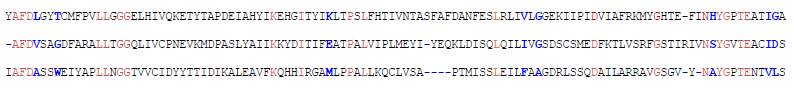
\includegraphics[width=1\textwidth]{poglavlja/5/slike/bakterije.png}
	\caption{A-domeni tri različite bakterije}
	\label{bakterije}
\end{figure}

Kako su biološke sekvence podložne promeni, umetanju i brisanju, čest je slučaj da $i$-ti simbol jedne sekvence odgovara simbolu na drugoj poziciji druge sekvence. U tom slučaju, cilj je postići najbolje poklapanje simbola.
Na primer, $ATGCATGC$ i $TGCATGCA$ nemaju delove koji se poklapaju, pa je njihova Hamingova udaljenost 8:

\begin{center}
$ATGCATGC$\\
$TGCATGCA$
\end{center}
    
Ali ako ih malo drugačije poravnamo, ove dve niske imaju 6 poklapajućih pozicija:

\begin{center}
$A\textcolor{black}{TGCATGC}-$\\
$-\textcolor{black}{TGCATGC}A$
\end{center}

Stringovi ATGCTTA i TGCATTAA imaju manje uočljive sličnosti:

\begin{center}
$A\textcolor{black}{TGC}-\textcolor{black}{TTA}-$\\
$-\textcolor{black}{TGC}A\textcolor{black}{TTA}A$
\end{center}

Ovi primeri navode nas da definišemo dobro poravnanje kao ono koje ima najveći mogući broj poklapanja. Povećanje broja poklapanja simbola možemo posmatrati kao igricu u kojoj u svakom potezu imamo dva izbora. Možemo da uklonimo oba simbola i osvojimo poen ako su oni isti ili možemo ukloniti simbol iz jedne od niski, ne osvojimo poene, ali omogućimo da u daljem igranju osvojimo više poena. Cilj je da maksimizujemo broj poena.


%%%%%%%%%%%%%%%%%%%%%%%% ALEX
\section{Igra poravnanja i najduža zajednička podsekvenca}

Kod \textbf{Igre poravnanja} cilj je ukloniti sve simbole iz sekvenci tako da pritom sakupimo što više poena :
\begin{itemize}
    \item Uklanjanje prvog simbola iz svake sekvence
         \begin{itemize}
         	\item \textcolor{black}{1} poen ako se simboli poklapaju,  \item\textcolor{black}{0} ako se simboli ne poklapaju
         \end{itemize}
    \item Uklanjanje prvog simbola iz jedne sekvence - 0 poena
\end{itemize}

\iffalse

\begin{figure}[h!]
\centering
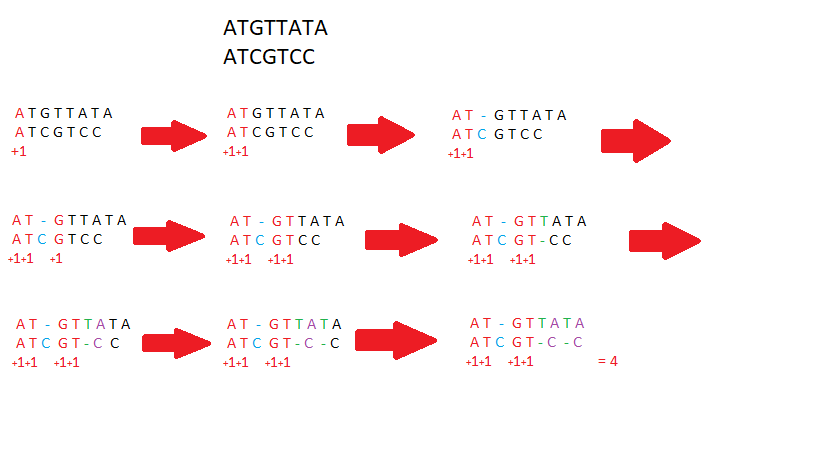
\includegraphics[width=0.7\textwidth]{poglavlja/5/slike/igraPoravnavanja.png}
\caption{Igra poravnanja}
\end{figure} 
\fi

\textbf{Poravnanje} dve sekvence predstavlja matricu koja ima dva reda. Prvi red matrice popunjen je simbolima prve sekvence (redom), drugi red matrice popunjen je simbolima druge sekvence (redom). Simboli razmaka ('-') mogu biti ubačeni u oba reda, bitno je da se dva takva simbola ne nađu u istoj koloni.

Poravnanje predstavlja jedan mogući scenario u kom se prva niska pretvara u drugu. Kolone koje sadrže karaktere sa istim karakterima, nazivamo poklapanje (match), a one sa različitim karakterima nazivamo promašaj (missmatch) i one predstavljaju zamenu jednog nukleotida drugim. Kolone koje sadrži razmake nazivamo indel-i: ako je razmak u prvom redu onda je u pitanju insercija, dok razmak u drugom redu predstavlja deleciju. Na slici \ref{slika:poravnavanje} vidimo 4 poklapanja, 2 promašaja, 1 inserciju i 2 delecije.

\begin{figure}[H]
\centering
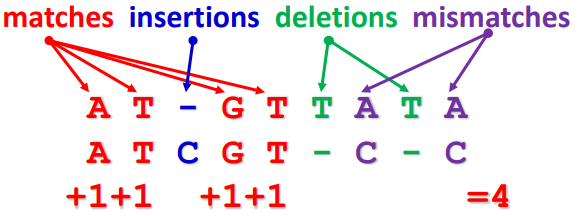
\includegraphics[width=0.4\textwidth]{poglavlja/5/slike/poravnanje.png}
\caption{Poravnanje}
\label{slika:poravnavanje}
\end{figure} 

Poklapanja (matches) u poravnanju dve sekvence ( u primeru \ref{slika:poravnavanje} to je ATGT) formiraju njihovu zajedničku podsekvencu (nije baš podniska jer se karakteri ne nalaze svi jedan do drugog). Želimo da imamo što više poklapanja odnosno želimo da imamo najdužu zajedničku podsekvencu.

\begin{tcolorbox}\textbf{Problem najduže zajedničke podsekvence.}
	Naći najdužu zajedničku podsekvencu dve niske. \\
	Ulaz: Dve niske. \\
	Izlaz: Najduža zajednička podsekvenca ovih niski
\end{tcolorbox}
%%%%%%%%%%%%%%%%%%%%%%%%%%%%%%%%%%%%%%%%%%%%

\section{Problem turiste na Menhetnu}

Zamislimo da smo turisti na Menhetnu, nalazimo se na uglu 59. ulice i 8. Avenije (gore levo) i želimo da stignemo do ugla 3. avenije i 42. ulice a da na putu prođemo što više znamenitosti. Pretpostavimo da se sve ulice seku pod pravim uglom. Mapu gradaa modelovaćemo grafom koji za svaku raskrsnicu sadrži čvor, a ulice su grane. Dodatno, želimo da za svaku granu dodamo broj koji će predstavljati broj znamenitosti koji se može videti u toj ulici. Želimo da pronađemo put u grafu od čvora (0, 0) - \textit{izvor}; do čvora (n, m) - \textit{ponor}; takav da je njegova vrednost najveća.

\noindent Pre svega postavimo problem:

\begin{tcolorbox}\textbf{Problem turiste na Menhetnu.}
	Naći najdužu putanju u pravougaonoj mreži gradskih ulica. \\
	Ulaz: Usmeren težinski mrežni graf. \\
	Izlaz: Najduža putanja od početnog (source) do krajnjeg čvora (sink) u mrežnom grafu. 
\end{tcolorbox}

Na slici \ref{slika:menhetn} grafički je prikazan problem turiste na Menhetnu. Cilj je stići od plavog do crvenog kruga i pri tom sakupiti što više poena. Dozvoljeno kretanje je dole i desno. Možemo koristiti pohlepni algoritam i tako doći do cilja. Ideja pohlepnog algoritma jeste da u svakom koraku bira granu koja je otežana najvećom vrednošću. Da li smo tako sakupili najviše poena?

\noindent Prikazali smo primer sa određenom topologijom grafa. Imali smo samo horizontalne i vertikalne grane usmerene na dosno odnosno na dole. Dodatna izmena grafa bi bila da imamo i neke dijagnalne grane (\ref{slika:menhetn3}).

\begin{minipage}{\textwidth}
	\centering
	\begin{minipage}{0.45\textwidth}
		\begin{figure}[H]
			\centering
			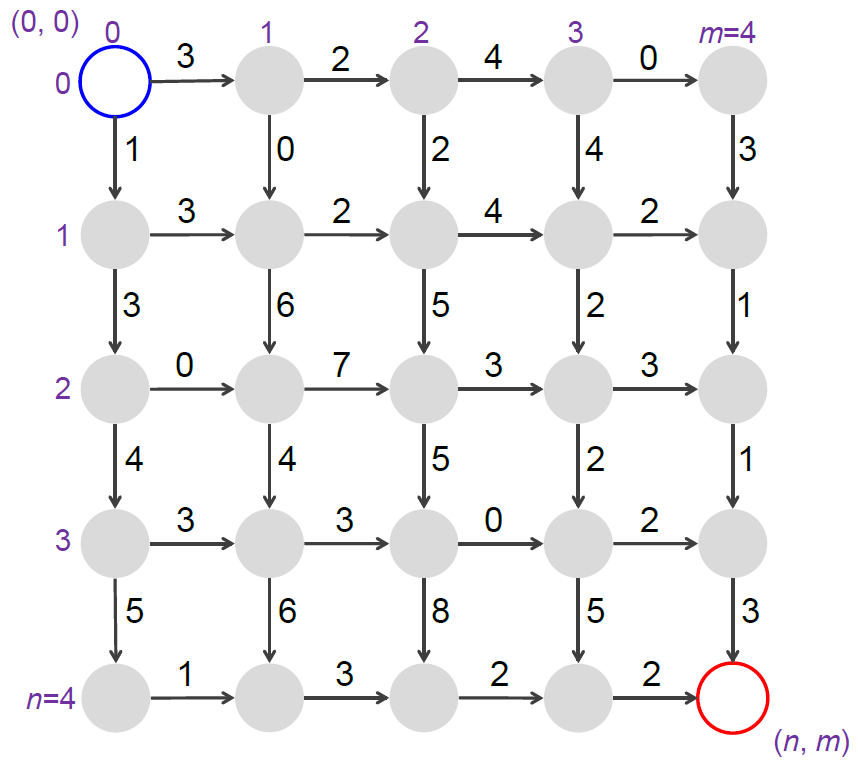
\includegraphics[width=\textwidth]{poglavlja/5/slike/menhetn2.png}
			\caption{Problem turiste na Menhetnu}
			\label{slika:menhetn}
		\end{figure}  
	\end{minipage}
	\hfill 
	\begin{minipage}{0.45\textwidth}
		\begin{figure}[H]
			\centering
			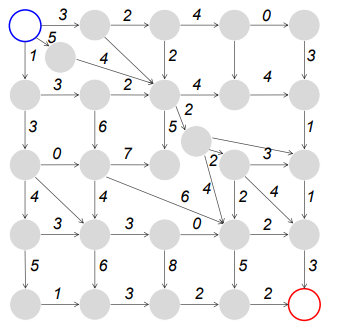
\includegraphics[width=\textwidth]{poglavlja/5/slike/menhetn3.png}
			\caption{Nepravilna mreža}
			\label{slika:menhetn3}
		\end{figure} 
	\end{minipage}
	\vspace*{1em}
\end{minipage}


\noindent Zbog toga definišemo problem za usmereni graf. Kasnije ćemo videti da nam neće odgovarati svaki usmereni graf.

\begin{tcolorbox}\textbf{Problem najduže putanje u usmerenom grafu.}
	Naći najdužu putanju između dva čvora u težinskom usmerenom grafu. \\
	Ulaz: Usmereni težinski graf sa označenim
čvorovima source i sink. \\
	Izlaz: Najduža putanja od čvora source do čvora
sink u usmerenom težinskom grafu. 
\end{tcolorbox}

Kakve veze ima turista i igra poravnanja? Mogli bismo svakoj koloni u matrici dodeliti jednu granu u grafu. Za poklapanje/promašaj dodajemo dijagonalne grane, za inserciju dodajemo horizontalnu, a za deleciju vertikalnu granu. Precizno uputsvo za izgradnju grafa dato je u sledećim koracima: 
\begin{itemize}
    \item Vrste označimo aminokiselinama iz prve niske
    \item Kolone označimo aminokiselinama iz druge niske
    \item U svaku presečnu tačku postavimo jedan čvor
    \item Gde god je moguće, postaviti vertikalne (insercija), horizontalne (delecija) i dijagonalne grane (match ili mismatch)
    \item Dijagonalne grane otežati koeficijentom 1, ostale koeficijentom 0
    \item Problem najduže zajedničke podsekvence se svodi na problem nalaženja najduže putanje između dva data čvora u usmerenom grafu
\end{itemize}

Poravnanje predstavlja jednu putanju od izvora do ponora. Kada nađemo poravnanje najvišeg skora našli smo i najdužu putanju u mrežnom grafu.

Dijagonalne crvene grane odgovaraju poklapanju simbola i imaju skor 1 (\ref{slika:poravnanje2}). Podsetimo se da je pronalaženje najduže zajedničke podsekvence dve niske ekvivalentno poravnanju tih niski sa maksimalnim brojem pogodaka. 

\begin{minipage}{\textwidth}
	\centering
	\begin{minipage}{0.45\textwidth}
		\begin{figure}[H]
			\centering
			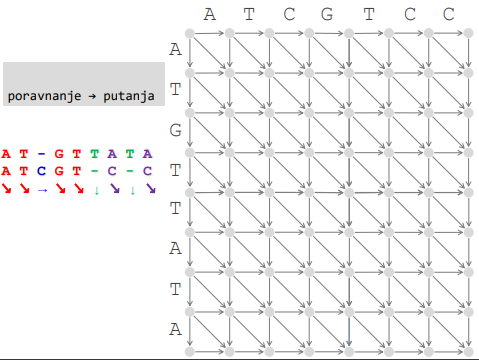
\includegraphics[width=\textwidth]{poglavlja/5/slike/menhetn4.png}
			\caption{Poravnanje $\rightarrow$ Putanja}
			\label{slika:menhetn4}
		\end{figure}  
	\end{minipage}
	\hfill 
	\begin{minipage}{0.45\textwidth}
		\begin{figure}[H]
			\centering
			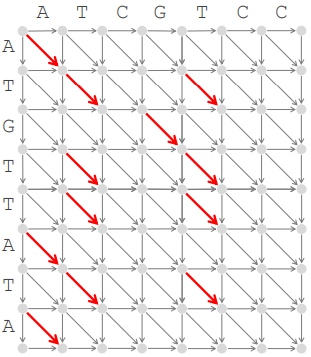
\includegraphics[width=\textwidth]{poglavlja/5/slike/poravnanje1.png}
			\caption{Poravnanje $\rightarrow$ Putanja}
			\label{slika:poravnanje2}
		\end{figure} 
	\end{minipage}
	\vspace*{1em}
\end{minipage}



\section{Problem kusura}

\noindent Upoznajmo se sa sledećim problemom:

\begin{tcolorbox}\textbf{Problem vraćanja kusura.}
	Naći minimalan broj novčića neophodnih za vraćanje kusura. \\
	Ulaz: Ceo broj $money$ i niz pozitivnih celih brojeva $(coin_1, coin_2, ..., coin_d)$. \\
	Izlaz: Minimalan broj novčića $(coin_1, coin_2, ..., coin_d)$ u apoenima koji rasitnjava sumu $money$. 
\end{tcolorbox}

\subsection{Pohlepni algoritam}

Najzastupljeniji način vraćanja kusura širom sveta podrazumeva iterativno traženje sledećeg najvećeg novčića. To bi značilo da bismo za kusur od 40 dinara dobili sledeće novčiće: 25 + 10 + 52. Ovakav način vraćanja kusura opisuje takozvani pohlepni algoritam. \\

\begin{lstlisting}
GreedyChange(money)
begin
    change %$\leftarrow$% empty collection of coins
	while money > 0
		coin %$\leftarrow$% largest denomination that does not exceed money
		add coin to change
		money %$\leftarrow$% money - coin
	return change
end
\end{lstlisting}

Međutim, ako malo bolje razmislimo ovo rešenje zapravo nije najbolje. Kusur bismo mogli vratiti i sa manje novčića na sledeći način: 40 = 20 + 20. \textbf{Zaključak}: GreedyChange ne daje optimalno rešenje!

\subsection{Rekurzivni algoritam}

Pokušajmo sada da problem rešimo na drugačiji način koristeći rekurziju. Za zadate apoene 6, 5, 1, koji je najmanji broj novčića neophodnih za vraćanje kusura od 9 centi?

\begin{figure}[h!]
\centering
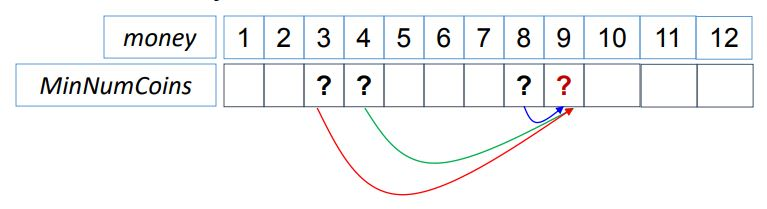
\includegraphics[width=0.7\textwidth]{poglavlja/5/slike/rekurzija1.JPG}
\caption{Vracanje kusura - rekurzija}
\label{slika:rekurzija}
\end{figure}

Problem rešavamo tako sto prvo od 9 oduzmemo 6 i dobijemo 3 kao ostatak kusura. Dakle, 9 se može vratiti od jednog novčića od 6 apoena i jos plus broj novčiča koji je potreban za preostali deo kusura od 3 centa. U istoj iteraciji analogno računamo za preostale apoene. Na slici \ref{slika:rekurzija} crvenim znakom pitanja označeno je traženo rešenje koje dobijemo rešavanjem manjih problema za kusure 3, 4 i 8. \\ 

MinNumCoins(9) = $\min$ 
$\begin{cases}$
$MinNumCoins(9-6) + 1 = MinNumCoins(3) + 1\\$
$MinNumCoins(9-5) + 1 = MinNumCoins(4) + 1\\$
$MinNumCoins(9-1) + 1 = MinNumCoins(8) + 1$
$\end{cases}$

~\\\noindent Na osnovu prethodnog, moguće je izvesti opštu formulu:

MinNumCoins(money) = $\min$ 
$\begin{cases}$
$MinNumCoins(money-coin_{1}) + 1 \\$
$\dots \\$
$MinNumCoins(money-coin_{d}) + 1 $
$\end{cases}$
\\
\noindent Hajde sada da vidimo kako bismo to isprogramirali:
\\
\begin{lstlisting}
RecursiveChange(money, coins)
begin
    if money = 0
        return 0
    MinNumCoins %$\leftarrow$% infinity 
    for i %$\leftarrow$% 1 to |coins|
        if money %$\geq coin_{i}$%
            NumCoins %$\leftarrow$% RecursiveChange(money - %$coin_{i}$%, coins)
            if numCoins + 1 < MinNumCoins
                MinNumCoins %$\leftarrow$% numCoins + 1
	return MinNumCoins
end
\end{lstlisting}

Reklo bi se da smo sada dobili odgovarajući algoritam za naš problem, hajde to da proverimo. Postavlja se pitanje, koliko je brz RecursiveChange? Pokušajmo na konkretnom primeru da dođemo do rešenja. Neka naš problem sada bude vraćanje kusura od 76 centi. Pomoću rekurzivnog stabla demonstrirajmo ponašanje našeg algoritma (\ref{slika:rekurzija2}).

\begin{figure}[h!]
\centering
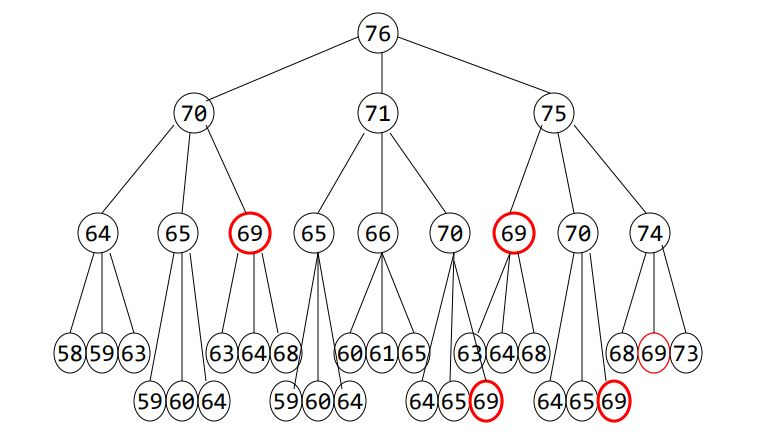
\includegraphics[width=0.7\textwidth]{poglavlja/5/slike/rekurzivnoStablo.JPG}
\caption{Vracanje kusura - ponašanje rekurzivnog algoritma}
\label{slika:rekurzija2}
\end{figure}

Ono što se odmah može primetiti jeste višestruko pozivanje algoritma za vrednost od 69 centi, čak 6 puta! Daljim procenama možemo doći do zaključka da se optimalna kombinacija novčića za 30 centi izračunava milijardama puta! Sada je očigledno da nam rekurzija ne rešava problem na najbolji mogući način.

\subsection{Vraćanje kusura dinamičkim programiranjem}

Cilj nam je da izbegnemo višestruka izračunavanja  vraćanja kusura za istu vrednost, tako da bi ideja bila da imamo objekat koji će pamtiti sva računanja i iz koga ćemo čitati već izračunate vrednosti. Dakle, umesto vremenski zahtevnih poziva  
\texttt{RecursiveChange(money - $coin_{i}$, coins)}, jednostavno bismo potražili vrednosti iz unapred izračunate tabele \textbf{MinNumCoins(money - $coin_{i}$)}.

\begin{lstlisting}
DPChange(money, coins)
begin
    MinNumCoins(0) %$\leftarrow$% 0 
    for m %$\leftarrow$% 1 to money
        MinNumCoins(m) %$\leftarrow$% infinity
        for i %$\leftarrow$% 1 to |coins|
            if m %$\geq coin_{i}$%
                if MinNumCoins(m - %$coin_{i}$%) + 1 < MinNumCoins(m)
                    MinNumCoins(m) %$\leftarrow$% MinNumCoins(m - %$coin_{i}$%) + 1
	return MinNumCoins(money)
end
\end{lstlisting}


\section{Dinamičko programiranje i putokazi za povratak}

Vratimo se na jednostavniji, Menhetn graf, koji nema dijagonalne grane. Pretpostavimo da do čvora sink možemo doći samo na dva načina: kretanjem južno $\downarrow$ ili kretanjem istočno $\rightarrow$. I dalje želimo da dođemo od izvora do ponora i to najdužom putanjom. Kako bismo to rešili rekurzivno? 

\iffalse 
\begin{figure}[h!]
\centering
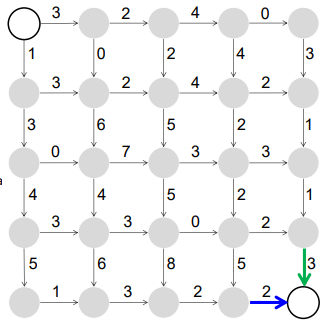
\includegraphics[width=0.7\textwidth]{poglavlja/5/slike/putokazi.png}
\caption{Južno ili istočno?}
\label{slika:putokazi}
\end{figure}
\fi 

\begin{lstlisting}
SouthOrEast(n, m)
if n=0 and m=0
    return 0
x %$\leftarrow$% -infinity, y %$\leftarrow$% -infinity
if n > 0
    x %$\leftarrow$% SouthOrEast(n-1,m)+weight of edge "%$\downarrow$%" into (n, m)
if m > 0
    y %$\leftarrow$% SouthOrEast(n,m-1)+ weight of edge "%$\rightarrow$%" into (n,m)
return max{x, y}
\end{lstlisting}

\noindent Nailazimo na isti problem kao kod rekurzivnog algoritma za vraćanje kusura. Ovaj algoritam se poziva za svaki čvor u grafu veličine $m\times n$, a pri tom se dešava da za jedan isti čvor računamo više puta. Zbog toga je ovaj pristup previše spor, pa prelazimo na dinamičko programiranje.

Krenućemo od početnog čvora. I prvo ćemo obraditi grane koje se nalaze na obodu grafa, a onda ćemo preći na ostale. Čvorovi na obodu su jednostavni jer imamo jedinstven put do njih. U svaki čvor $(i, j)$ upisujemo dužinu maksimalne putanje od $(0,0)$ do $(i,j)$. Ostale čvorove obrađujemo kolonu po kolonu. Za svaki čvor $(i, j)$, koji se ne nalazi na obodu, biramo da li ćemo do njega doći sa severa ili sa zapada. Naravno, odabir zavisi od težine grana koje vode do čvora, pri čemu se bira veća vrednost. Može se desiti da nam obe grane daju istu vrednost akda je sve jedno koju ćemo odabrati.

\begin{minipage}{\textwidth}
	\centering
	\begin{minipage}{0.4\textwidth}
		
		\begin{figure}[H]
			\centering
			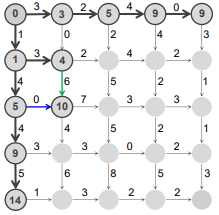
\includegraphics[width=\textwidth]{poglavlja/5/slike/putokazi1.png}
			\caption{Računanje vrednosti puta za svaki čvor.}
			\label{slika:putokazi1}
		\end{figure}  
	\end{minipage}
	\hfill 
	\begin{minipage}{0.4\textwidth}
		\begin{figure}[H]
			\centering
			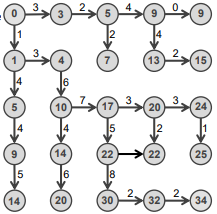
\includegraphics[width=\textwidth]{poglavlja/5/slike/putokazi3.png}
			\caption{Cene za svaki čvor su određene, odabrane grane su podebljane.}
			\label{slika:putokazi3}
		\end{figure} 
	\end{minipage}
	\vspace*{1em}
\end{minipage}


\iffalse
\begin{figure}[h!]
\centering
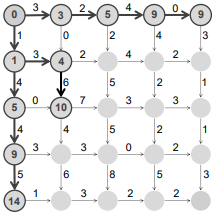
\includegraphics[width=0.5\textwidth]{poglavlja/5/slike/putokazi2.png}
\caption{Južno ili istočno?}
\label{slika:putokazi2}
\end{figure}
\fi 



Na slici \ref{slika:putokazi3} prikazane su podebljane grane koje predstavljaju putokaze za povratak od čvora sink do čvora source. 


Sve ovo treba predstaviti matematički, a to najlakše možemo učiniti rekurentnom relacijom. Označimo sa $s_{i, j}$ dužinu najduže putanje od izvora do čvora $(i, j)$. Onda važi sledeća rekurentna relacija:

$s_i,_j$ = $\max$ $\begin{cases}$
$s_{i-1},_j +$ weight of edge $"\downarrow"into (i,j)\\$
$s_i,_{j-1} +$ weight of edge $"\rightarrow"into (i,j)$
$\end{cases}$


Na osnovu ove rekurentne relacije lako možemo napisati algoritam koji rešava problem turiste na Menhetnu.

\begin{lstlisting}
ManhattanTourist(n, m, Down, Right)
%$s_0,_0$% %$\leftarrow$% 0
for i %$\leftarrow$% 1 to n
    %$s_i,_0$% %$\leftarrow$% %$s_{i-1},_0$% + %$down_i,_0$%
for j %$\leftarrow$% 1 to m
    %$s_0,_j$% %$\leftarrow$% %$s_0,_{j-1}$% + %$right_0,_j$% 
for i %$\leftarrow$% 1 to n
    for j %$\leftarrow$% 1 to m
        %$s_i,_j$% %$\leftarrow$% %$\max$% { %$s_{i-1},_j$% + %$down_i,_j$%, %$s_i,_{j-1}$% + %$right_i,_j$% }
return %$s_n,_m$%
\end{lstlisting}



\section{Od Menhetna do grafa poravnanja }

Prikazali smo kako se dinamičko programiranje može primeniti na Menhetn graf. Međutim, ono što nama zaista treba jeste algoritam koji će raditi sa grafom poravnanja. Osim horizontalnih i vertikalih grana, u grafu poravnanja imamo i dijagonalne grane. Pored toga, za dijagonalnu granu moramo razlikovati situacije kada se desilo poklapanje i kada se desio promašaj. Rekurentna relacija dinamičkog programiranja kod grafa poravnanja u opštem slučaju bi bila:

$s_i,_j$ = $\max$ $\begin{cases}$
$s_{i-1},_j$ + 
$weight\ of\ edge\ "\downarrow"\ into\ (i,j)\\$
$s_i,_{j-1}$ + 
$weight\ of\ edge\ "\rightarrow"\ into\ (i,j)\\$
$s_{i-1},_{j-1}$ + 
$weight\ of\ edge\ "\searrow"\ into\ (i,j)$
$\end{cases}$

Kada bismo hteli da otežamo grane u skladu sa prethodnim pristupom, odnosno da poklapanje nosi vrednost 1, a ostalo 0, dobili bismo sledeću rekurentnu realciju:

$s_i,_j$ = $\max$ $\begin{cases}$
$s_{i-1},_j + 0\\$
$s_i,_{j-1} + 0\\$
$s_{i-1},_{j-1} + 1, v_i = w_j\\$
$s_{i-1},_{j-1} + 0, v_i \neq w_j$
$\end{cases}$

Crvene grane imaju težinu 1, a ostale grane težinu 0.

\iffalse 
\begin{figure}[h!]
\centering
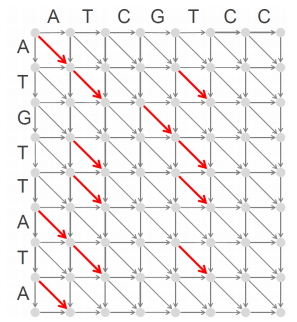
\includegraphics[width=0.5\textwidth]{poglavlja/5/slike/graf1.png}
\caption{ Crvene grane težina 1, ostale grane težina 0, $v_i$ i $w_j$ oznake vrste i kolone}
\label{slika:povratak}
\end{figure}
\fi 

Na slici \ref{slika:backtrack} se vide boldovane grane koje su nastale primenom pravila rekurentne relacije. One predstavljaju putokaze za povratak (backtrack) kod grafa za najdužu zajedničku podsekvencu. 

\begin{figure}[h!]
\centering
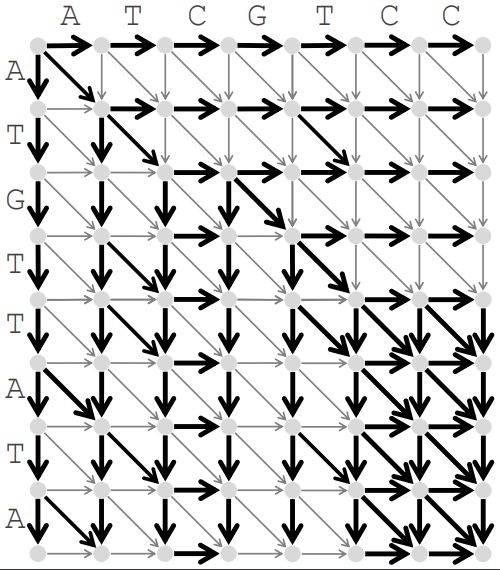
\includegraphics[width=0.5\textwidth]{poglavlja/5/slike/backtrack.png}
\caption{Putokazi za povratak (backtrack)}
\label{slika:backtrack}
\end{figure}

\subsection{Računanje putokaza za povratak }

Kada bismo sproveli isti pristup kao kod Menhetn grafa i kada bismo beležili grane koje smo birali, i ovde bismo da te grane koristimo kao putokaze i dođemo od ponora do izvora odnosno mogli bismo da rekonstruišemo najdužu putanju. Razlika je što ovde ima više podebljanih grana, tj. putokaza, što nam govori i da postoji više puteva koji imaju maksimalnu vrednost.

Ako nam je $s_{i, j}$ dato prethodno definisanom rekurentnom relacijom, putokaze možemo računati preko sledeće rekurentne relacije:

$backtrack_i,_j$  $\leftarrow$  $\max$ $\begin{cases}$
$"\rightarrow", s_i,_j = s_{i},_{j-1}\\$
$"\downarrow", s_i,_j = s_{i-1},_j\\$
$"\searrow", otherwise$
$\end{cases}$


Podsetimo se sada kako bismo rekontruisali putanju preko putokaza kod Menhetn grafa? Krenuli bismo od krajnjeg čvora (sink) i pratili putokaze u obrnutom smeru do početnog čvora (source). Na slici \ref{slika:backNZPS} možemo videti povratak (backtracking) kod grafa za najdužu zajedničku podsekvencu.
\iffalse 
\begin{figure}[h!]
\centering
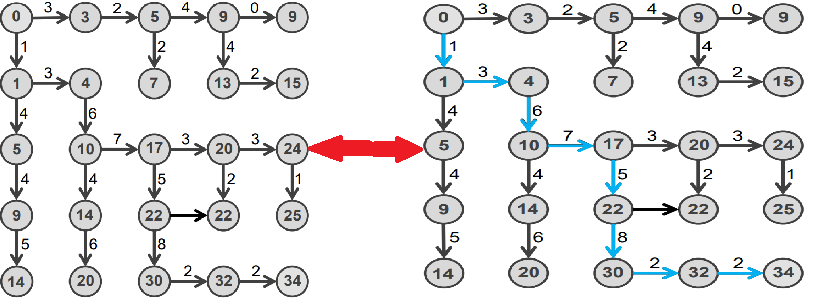
\includegraphics[width=0.7\textwidth]{poglavlja/5/slike/rek3.png}
\caption{Rekonstrukcija putanje preko putokaza kod Menhetn grafa}
\label{slika:rek3}
\end{figure}
\fi 

\begin{figure}[h!]
\centering
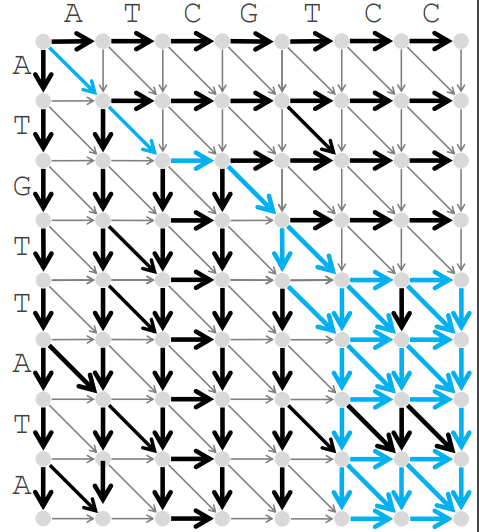
\includegraphics[width=0.4\textwidth]{poglavlja/5/slike/backtrackNajduzaZajPS.png}
\caption{Backtracking}
\label{slika:backNZPS}
\end{figure}

U nastavku je dat pseudokod za određivanje najduže zajedničke podsekvence (LCS – longest common subsequence) korišćenjem putokaza za povratak.

\begin{lstlisting}
OutputLCS (backtrack, v, i, j)
if i = 0 or j = 0
    return
if %$backtrack_i,_j$% = "%$\rightarrow$%"
    OutputLCS (backtrack, v, i, j-1)
else if %$backtrack_i,_j$% = "%$\downarrow$%"
    OutputLCS (backtrack, v, i-1, j)
else
    OutputLCS (backtrack, v, i-1, j-1)
    output  %$v_i$%
\end{lstlisting}


Do sada smo pretpostavljali da graf u kom tražimo najdužu putanju ima samo tri vrste grana. Da li se OutputLCS može generalizovati tako da važi i za grafove koji nemaju tako specifičnu
topologiju? Kako se rekurentna relacija dinamičkog programiranja menja za ovakav graf? \ref{slika:rekRel}
\begin{figure}[h]
\centering
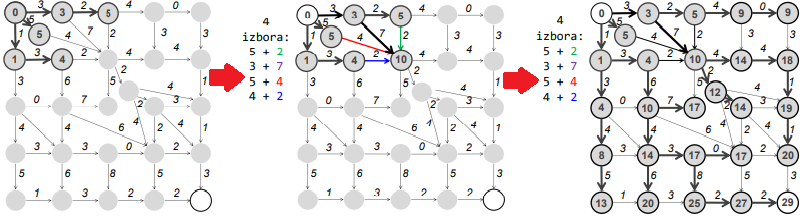
\includegraphics[width=\textwidth]{poglavlja/5/slike/rekurentaRelDinProg.png}
\caption{Prikaz algoritma na opštem usmerenom težinskom grafu}
\label{slika:rekRel}
\end{figure}
\\

\noindent\textit{$s_a$ = $max_{all\ predecessors\ b\ of\ node\ a}$\{$s_b$+ weight of edge from b to a\}}


\begin{figure}[h]
\centering
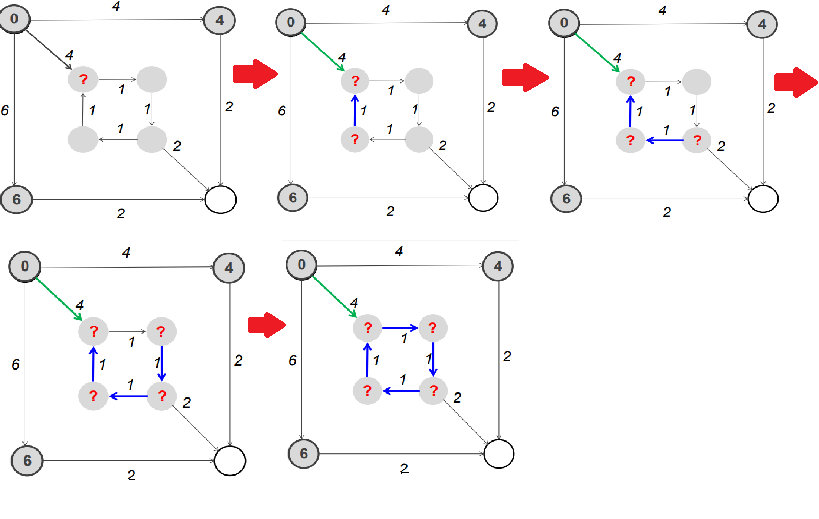
\includegraphics[width=0.7\textwidth]{poglavlja/5/slike/racunanje.png}
\caption{Računanje skora za SVE prethodnike}
\label{slika:racunanje}
\end{figure}


Kod ovakve rekurentne relacije, važno je da pri računanju $s_a$ imamo izračunate $s_b$ za sve čvorove prethodnike b (čvorovi za koje postoji grana do čvora a) Da li je to moguće u bilo kom usmerenom težinskom grafu? Odgovor je \textbf{nije}. Da bismo kod svakog čvora mogli da izračunamo skor za sve njegove prethodnike, usmereni težinski graf mora biti acikličan - DAG (Directed Acyclic Graph). 

Ako je dat usmereni aciklični graf, da li njegove čvorove možemo poređati u niz tako da njihov redosled u nizu osigurava uslov da pri računanju $s_a$ imamo izračunate $s_b$ za sve čvorove prethodnike b (čvorovi za koje postoji grana do čvora a)? Odgovor je \textbf{da}, moguće je poređati sve čvorove grafa u niz i taj niz topološki sortirati.
\\
\\
\noindent\textbf{Topološko sortiranje} : Sortiranje čvorova DAG-a u nizu tako da sve grane u takvom nizu idu s leva na desno. \\
\textbf{ Teorema}: Svaki DAG se može topološki sortirati.
\\\\
Topološko sortiranje svakog DAG-a se obavlja za O(\#edges) koraka. Kada imamo topološko sortiranje čvorova, možemo odrediti najužu putanju od izvora do ponora tako što ćemo proći čvorove u redosledu koji diktira topološko sortiranje.  Algoritam za nalaženje najduže putanje u DAG-u dat je u nastavku.

\begin{lstlisting}
LongestPath(Graph, source, sink)
for each node a in Graph
     %$s_a$% %$\leftarrow$% -%$\infty$%
%$s_{source}$% %$\leftarrow$%  0
topologically order Graph
for each node a (from source to sink in topological order)
%$s_a$%  %$\leftarrow$% %$max_{all\ predecessors\ b\ of\ node\ a}$% {%$s_b$% + weight of edge from b to a}
return %$s_{sink}$%
\end{lstlisting}

Pošto svaka grana učestvuje tačno jednom, složenost je O(\#edges). LongestPath vraća dužinu najdužeg zajedničkog podniza ali ne rekonstruiše putanju.

~
\section{Od globalnog do lokalnog poravnanja}

Do sada smo podrazumevali da dužine niski koje poredimo ne odstupaju previse jedna od druge (da ne poredimo nisku od npr. 10 sa niskom od 100 karaktera). Ako to podrazumevamo, onda radimo globalno poravnanje. Međutim, i druga situacija je moguća, ali moramo malo izmeniti pristup problemu i bliže ga razmotriti.

Do, sada, skor poravnanja računali smo kao broj poklapanja - $matches$. Međutim, u slučaju kada su niske potpuno različitih dužina, ovaj način računanja skora neće biti sasvim prikladan, moraćemo da ga malo profinimo. Dakle, do sad je poklapanje nosilo 1, a ostale situacije vrednost 0. Sada, uvodimo kazne za nepoklapanje ($\mu$) i za indel-e($\sigma$). Skor sa mismatch i indel kaznama računamo po formuli $matches - \mu * mismatches - \sigma * indels$ 


U primeru koji je dat prilikom opisa igre poravnanja, skor je bio 4. Primenom nove formule dobijamo skor -7. 

Uvodimo pojam matrice skora. Vrste (odnosi se na karaktere prve niske) i kolone (odnosi se na karaktere druge niske) označimo vrednostima karaktera iz azbuke i praznim simbolom. Elementi matrice imaju vrednosti kazne za svaku kombinaciju karaktera. Na dijagonali će se naći jedinice jer tada dolazi do poklapanja, poslednja vrsta i kolona imaju vrednost -$\sigma$ jer su to indel-i, a ostale vrednosti su promašaji pa su vrednosti -$\mu$.

Možemo napraviti generalniju matricu, gde možemo uvesti dodatne vrednosti za različita nepoklapanja. Ovaka matrica se može odrediti eksperimentalno. Posmatra se koje mutacije se dešavaju često, koje ređe i na osnovu toga određujemo skor za različite kombinacije. Primer je dat na slici \ref{slika:matriceSkora}.

\begin{figure}[h]
	\centering
	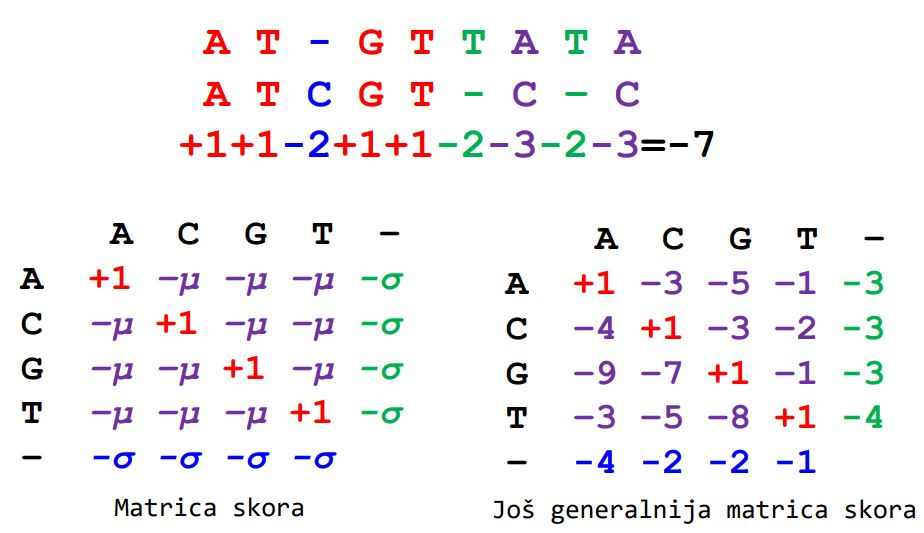
\includegraphics[width=0.9\textwidth]{poglavlja/5/slike/matriceSkora.JPG}
	\caption{Matrica skora}
	\label{slika:matriceSkora}
\end{figure}

Matrica skora može se definisati i za proteinske sekvence i tu možemo videti koliko se često dešava da jedna aminokiselina mutira u drugu. Postoji više vrsta ovakvih matrica za proteinske sekvence.

U okviru algoritma dinamičkog programiranja bila je u fokusu rekurentna relacija koja je rešavala problem. Hajde i sada da odredimo rekurentnu relaciju koja će nam rešiti problem. Počinjemo od prethodno definisane rekurentne relacije:

$s_i,_j$ = $\max$ $\begin{cases}$
$s_{i-1},_j$ + 
$\textcolor{black}{weight\ of\ edge\ "\downarrow"\ into\ (i,j)}\\$
$s_i,_{j-1}$ + 
$\textcolor{black}{weight\ of\ edge\ "\rightarrow"\ into\ (i,j)}\\$
$s_{i-1},_{j-1}$ + 
$\textcolor{black}{weight\ of\ edge\ "\searrow"\ into\ (i,j)}$
$\end{cases}$

\begin{figure}[!htb]
	\begin{minipage}{0.49\textwidth}
		\noindent Umesto 0, dodajemo negirano $\sigma$ ili $\mu$: \\
		\\
		$s_i,_j$ = $\max$ $\begin{cases}$
		$\textcolor{black}{s_{i-1},_j - \sigma}\\$
		$\textcolor{black}{s_i,_{j-1} - \sigma}\\$
		$\textcolor{black}{s_{i-1},_{j-1} + 1, v_i = w_j}\\$
		$\textcolor{black}{s_{i-1},_{j-1} - \mu, v_i \neq w_j}$
		$\end{cases}$
	\end{minipage}
	\hfill
	\begin{minipage}{0.49\textwidth}
	    Isto možemo zapisati pomoću funkcije \texttt{score()}, koja je zgodna ako imamo generalniju matricu skora: \\
		\\
		$s_i,_j$ = $\max$ $\begin{cases}$
		$\textcolor{black}{s_{i-1},_j + score(v_i, -)}\\$
		$\textcolor{black}{s_i,_{j-1} + score(-, w_j)}\\$
		$\textcolor{black}{s_{i-1},_{j-1} score(v_i, w_j)}\\$
		$\end{cases}$
	\end{minipage}
\end{figure}

\iffalse 
\begin{figure}[!htb]
     \begin{minipage}{0.49\textwidth}
        
     \end{minipage}
     \hfill
     \begin{minipage}{0.49\textwidth}
     	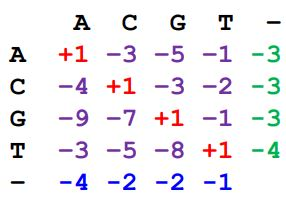
\includegraphics[width=\linewidth]{poglavlja/5/slike/rekurentna.JPG}
     	\caption{}\label{}
     \end{minipage}
   \end{figure}
\fi    

Podsetimo se problema globalnog poravnanja.
\begin{tcolorbox}\textbf{Problem globalnog poravnanja.}
	Naći poravnanje sa najvišim skorom između dve niske za datu matricu skora. \\
	Ulaz: Niske v i w, kao i matrica skora score \\
	Izlaz: Poravnanje niski v i w čiji je skor poravnanja (prema matrici skora) maksimalan od svih mogućih poravnanja v i w. 
\end{tcolorbox}


Zbog čega uopšte razmatramo druga poravnanja? Rekli smo da ćemo nekada želeti da poredimo niske različitih dužina odnosno, neku malu u odnosno na neku priličnu veliku sekvencu. 

Ograničenja globalnog poravnanja su \textbf{homeobox geni}. Analiza homeobox gena daje primer problema za koji globalno poravnanje neće uspeti da otkrije biološki bitne sličnosti. Ovi geni regulišu razvoj embriona i prisutni su kod velikog broja vrsta, od muva do ljudi. Homobox geni su dugački i veoma se razlikuju od vrste do vrste, ali postoje veoma kratki regioni, koje nazivamo \textbf{homeodomeni}, koji su čvrsto konzervirani. Ukoliko bismo pokušali da prnađemo taj kratak homeodomen kod dve različite vrste. Dva gena u različitim vrstama mogu biti slična u kratkim, konzerviranim regionima, a različita u ostalim delovima. Homeobox geni sadrže kratak region homeodomen koji je čvrsto konzerviran među različitim vrstama. Globalno poravnanje može da propusti nalaženje homeodomena jer pokušava da poravna sekvence u celosti. Uporedimo sledeća dva poravnanja: 

\begin{figure}[!htb]
 \begin{minipage}{0.49\textwidth}
    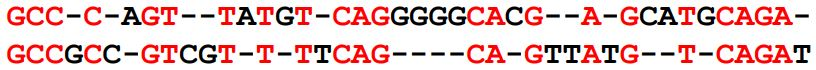
\includegraphics[width=\linewidth]{poglavlja/5/slike/globalno.JPG}
   \caption{Globalno poravnanje}
   \label{globalno}
   score = 22(matches) - 2(indent) = 2
 \end{minipage}
 \hfill
 \begin{minipage}{0.49\textwidth}
   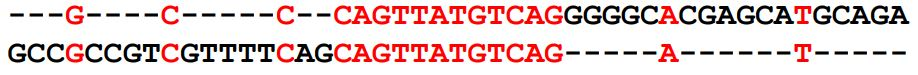
\includegraphics[width=\linewidth]{poglavlja/5/slike/lokalno.JPG}
   \caption{Lokalno poravnanje}
   \label{lokalno}
   score = 17 (matches) - 30(indent) = -13
 \end{minipage}
\end{figure}

\iffalse 
\begin{figure}[!htb]
 \begin{minipage}{0.49\textwidth}
    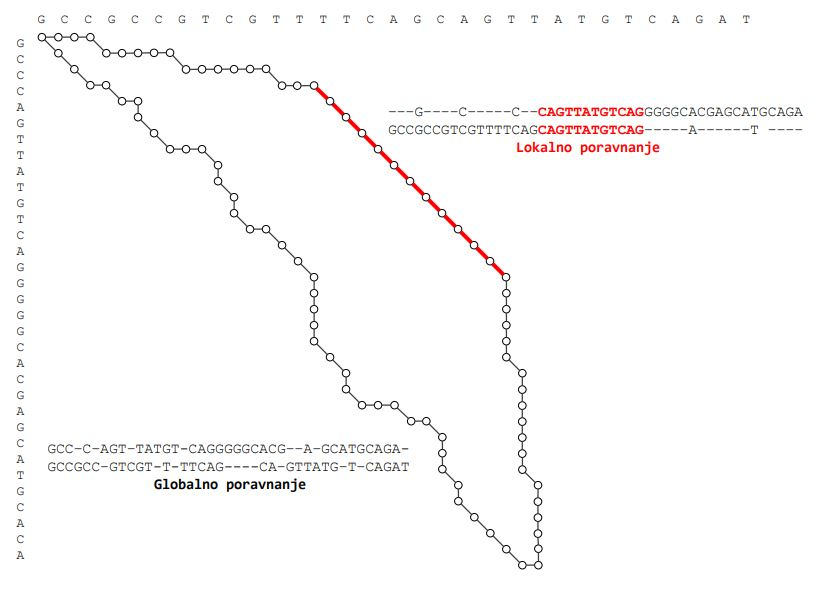
\includegraphics[width=\linewidth]{poglavlja/5/slike/grafik_poravnanje1.JPG}
   \caption{}\label{}
 \end{minipage}
 \hfill
 \begin{minipage}{0.49\textwidth}
   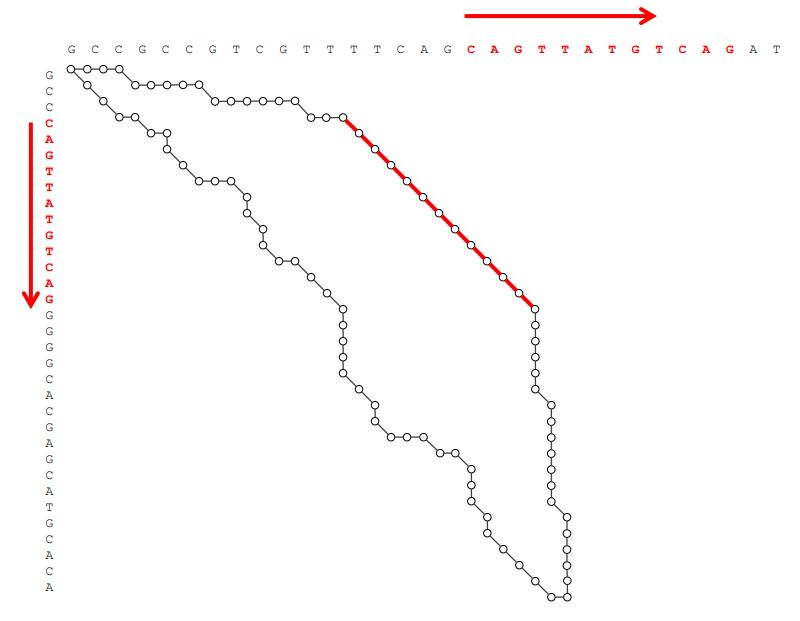
\includegraphics[width=\linewidth]{poglavlja/5/slike/grafik_poravnanje2.JPG}
   \caption{}\label{}
 \end{minipage}
\end{figure}
\fi 

\noindent Vidimo da poravnanje na slici \ref{lokalno} ima 17 poklapanja (u odnosu na 22, na slici \ref{globalno}), i ima čak 30 indel-1 (dok na prvoj ima 20). Skor je dosta lošiji, iznosi '13, u odnosu na 2. Međutim, \ref{lokalno} poravnanje ima dugačak zajednički deo koji se poklapa, pronašli smo kratak konzervirani region. Tako da, ako se zapitamo koje od ovih poravnanja je bolje, iz priloženog zaključujemo da je to lokalno poravnanje.


Kada su biološki bitne sličnosti prisutne u nekim delovima sekvenci \texttt{v} i \texttt{w} i odsutne u ostalim, bilozi pokušavaju da ignorišu globalno poravnanje i umesto toga poravnaju podniske  \texttt{v} i \texttt{w}, čime se dobija lokalno poravnanje ovih niski. Problem pronalaženja podniski koje maksimizuju skor globalnog poravnanja naziva se \textbf{Problem lokalnog poravnanja}.


\subsection{Lokalno poravnanje}

Lokalno poravnanje računamo kao globalno poravnanje u pravougaoniku, pogledajmo sliku \ref{slika:pravougaonici}. Odnosno, tražimo neke delove niske u kojima ćemo tražiti pokalapanja umesto u celoj niski.

\begin{figure}[H]
 \begin{minipage}{0.35\textwidth}
    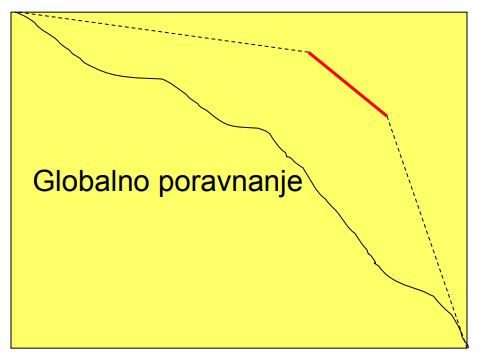
\includegraphics[width=\linewidth]{poglavlja/5/slike/lokalno_poravnanje_pravougaonici1.JPG}
   \caption{}\label{}
 \end{minipage}
 \hfill
 \begin{minipage}{0.45\textwidth}
   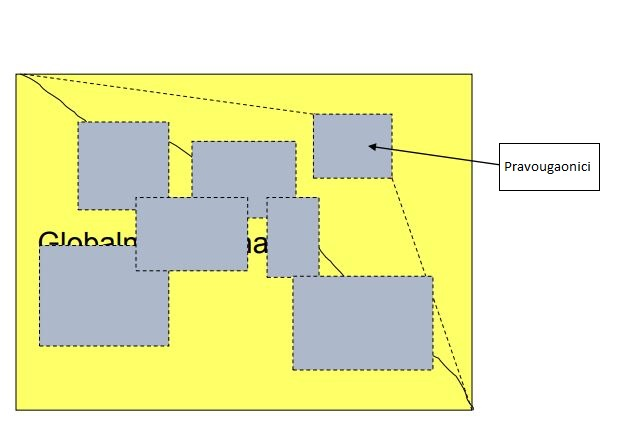
\includegraphics[width=\linewidth]{poglavlja/5/slike/lokalno_poravnanje_pravougaonici2.JPG}
   \caption{}\label{slika:pravougaonici}
 \end{minipage}
\end{figure}

\noindent Da bismo dobili lokalno poravnanje potrebno je da izračunamo globalno poravnanje u okviru svakog pravougaonika. Algoritam lokalnog poravnanja ponovićemo između svaka dva čvora, ne samo između početnog (source) i krajnjeg (sink), što radimo za globalno poravnanje. Stoga, broj ponavljanja algoritma će biti $\#nodes ^ 2$ puta. 

\begin{tcolorbox}\textbf{Problem lokalnog poravnanja.}
	Naći lokalno poravnanje najvećeg skora između dve niske. \\
	Ulaz: Niske v i w, kao i matrica skora score \\
	Izlaz: Podniske niski v i w čije je globalno poravnanje (prema matrici skora) maksimalno među svim globalnim poravnanjima svih podniski niski v i w. 
\end{tcolorbox}


\subsubsection{Besplatna taksi vožnja}

\iffalse 
\begin{figure}[H]
\centering
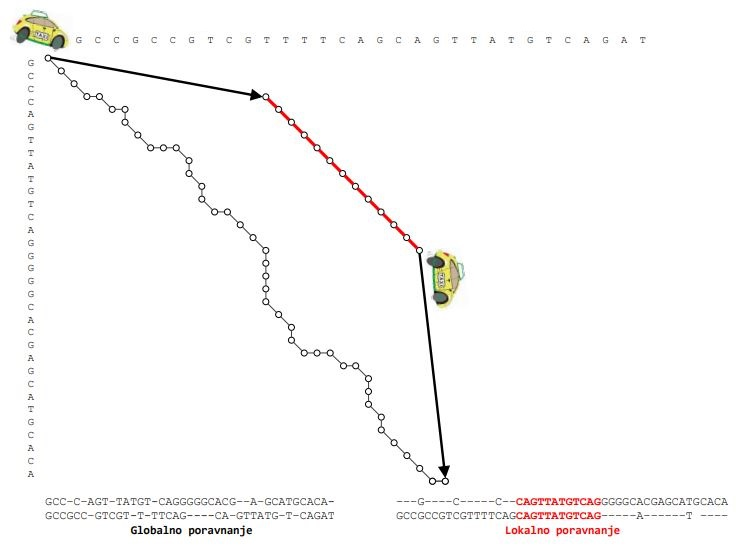
\includegraphics[width=0.7\textwidth]{poglavlja/5/slike/free_taxi.JPG}
\caption{Besplatne taksi vožnje}
\label{slika:taksiFree}
\end{figure} 
\fi 

\begin{figure}[H]
     \begin{minipage}{0.39\textwidth}
        Kako ovo možemo da realizujemo? Zamislimo da postoji taksi koji bi nas besplatno vozio do tačke početka lokalnog poravnanja, i od tačke završetka lokalnog poravnanja pa do kraja. Na taj način ne bismo skupili negativne poene dok ne pronađemo odgovarajući pravougaonik , već samo pozitivne. Ovakva vožnja nam daje samo skor lokalnog poravnanja kao što smo i želeli. Kako bi izgledao Menhetn graf za naš problem? Dodamo grane težine 0 od (0,0) do svakog čvora, i od svakog čvora do (n,m). Ukupan broj dodatih grana je $O(|v|+|w|)$, pa algoritam ostaje brz.
     \end{minipage}
     \hfill
     \begin{minipage}{0.49\textwidth}
       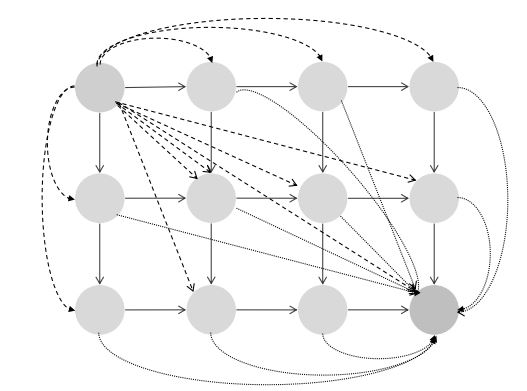
\includegraphics[width=\linewidth]{poglavlja/5/slike/free_taxi_graf.JPG}
       \caption{Menhetn graf za lokalno poravnanje}\label{}
    \end{minipage}
\end{figure}


Zahvaljujući besplatnoj vožnji, ne moramo da tražimo najduži put između svaka dva čvora u grafu. Ukupan broj grana u grafu je $O(|v| \cdot |w|)$, što je i dalje malo. Pošto vreme izvršavanja zavisi od broja grana, ovaj algoritam biće brz. Što se tiče računanja vrednosti $s_{i, j}$, dodavanje grana težine 0 od čvora $(0, 0)$ do svakog čvora čini izvor prethodnikom svih čvorova. Zato, sada imamo četiri grane koje ulaze u čvor $(i, j)$, a rekurentna relacija se samo proširuje jednim elementom:

$s_i,_j$ = $\max$ $\begin{cases}$
$0\\$
$s_{i-1},_j$ + 
$\textcolor{black}{weight\ of\ edge\ "\downarrow"\ into\ (i,j)}\\$
$s_i,_{j-1}$ + 
$\textcolor{black}{weight\ of\ edge\ "\rightarrow"\ into\ (i,j)}\\$
$s_{i-1},_{j-1}$ + 
$\textcolor{black}{weight\ of\ edge\ "\searrow"\ into\ (i,j)}$
$\end{cases}$
\\
\\
Takođe, pošto smo dodali grane od svakog čvora do ponora, svaki čvor predstavlja prethodnika ponora pa će najveća vrednost $s_{n, m}$ najvećoj vrednosti iz matrice.

\iffalse
\begin{figure}[H]
     \begin{minipage}{0.59\textwidth}
     \end{minipage}
     \hfill
     \begin{minipage}{0.39\textwidth}
       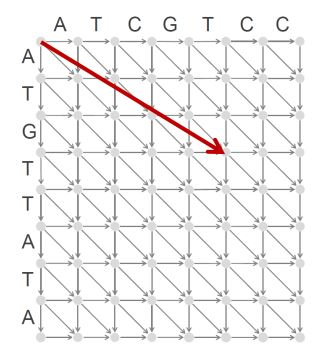
\includegraphics[width=\linewidth]{poglavlja/5/slike/lokalno_poravnanje_0.JPG}
       \caption{weight of (0,0) into (i,j) = 0}\label{}
    \end{minipage}
\end{figure}
\fi 

\subsection{Kažnjavanje praznina}

U globalnom poravnanju je fiksna kazna $\sigma$ bila dodeljena svakom indel-u. Međutim, ova fiksna kazna može biti preoštra kod lokalnog poravnanja kada možemo imati 100 uzastopnih indel-a. Niz od k uzastopnih indel-a često predstavlja jedan isti evolucioni događaj, ne k različitih, (\ref{slika:kaznjavanje}). Šta to znači? Pretpostavlja se da kada se jedna vrsta razdvajala od druge, znači da se tih k indel-a odjednom dogodilo, a ne u više navrata. Zbog toga uvodimo afinu kaznu za praznine (skup uzastopnih crtica).

\begin{figure}[h]
\centering
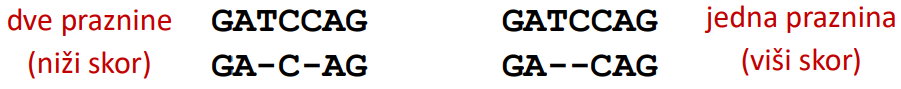
\includegraphics[width=0.5\textwidth]{poglavlja/5/slike/kaznjavanjePraznina.png}
\caption{}
\label{slika:kaznjavanje}
\end{figure}


\textbf{Afina kazna} za prazninu dužine k definisana je formulom $\sigma+\varepsilon*(k-1)$, gde je 
\begin{itemize}
    \item $\sigma$ kazna za \textbf{otvaranje} praznine
    \item $\varepsilon$ kazna za \textbf{proširenje} praznine
    \item $ \sigma > \varepsilon$ , jer otvaranje praznine treba kazniti više nego njeno proširenje
\end{itemize}

Kako ćemo to modelovati grafom? Na slici \ref{slika:modelovanje} prikazano je modelovanje afinih kazni za praznine pomoću dugih grana.

\begin{figure}[h!]
\centering
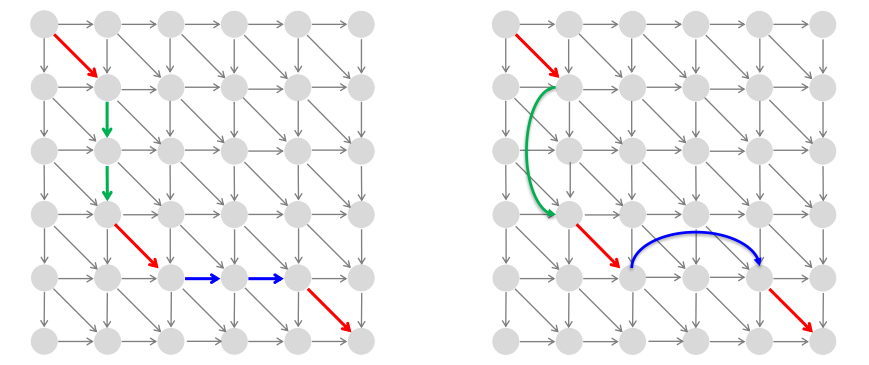
\includegraphics[width=0.7\textwidth]{poglavlja/5/slike/modelovanjePomocuDugihGrana.png}
\caption{Modelovanje afinih kazni za praznine pomoću dugih grana}
\label{slika:modelovanje}
\end{figure}

\subsection{Izgradnja Menhetn grafa sa afinim kaznama za praznine}

Dodajemo nove grane za sve nesusedne čvorove sa dužinama $\sigma + \varepsilon \cdot k$. Pre ovoga smo imali kvadratni broj grana, sada smo prešli na kub.

\begin{figure}[h!]
\centering
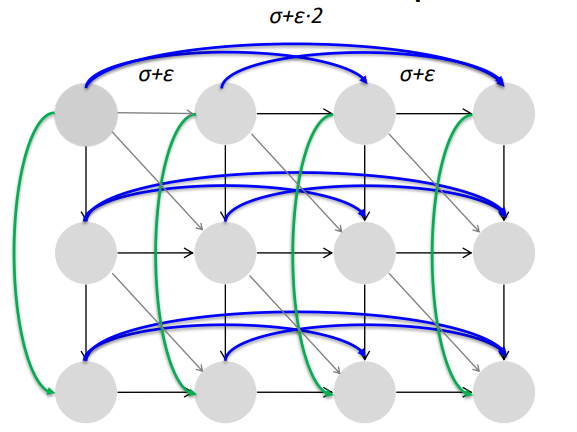
\includegraphics[width=0.5\textwidth]{poglavlja/5/slike/MenhettnAifnePraznine.png}
\caption{Dodali smo $O(n^3)$ grana}
\label{slika:afiniMenhetn}
\end{figure}

Vremenska složenost je direktno proporcionalna broju grana, zbog čega želimo da smanjimo broj grana u grafu (trenutno je $O(n^3)$, \ref{slika:afiniMenhetn}). Jedan način za smanjivanje broja grana je povećanje broja čvorova u grafu. Zato delimo Menhetn graf na tri nivoa (\ref{slika:simulacija}).

Kada smo pravili Menhetn graf, dodavali smo grane horizontalno, vertikalno i dijagonalno, gde god je to bilo moguće. Sada želimo da razdvojimo sve to, tako da donji nivo sadrži samo vertikalne (insercije), srednji samo dijagonalne (poklapanje/promašaj) i gornji nivo sadrži samo horizontalne grane (delecija).

Kako se ponašamo sad prikazano je na slici \ref{slika:simulacija}. Prelazak sa gornjeg ili donjeg nivoa na srednji ima cenu nula (zatvaranje praznine, besplatna taksi vožnja), dok prelazak sa srednjeg na gornji ili donji ima vrednost $\sigma$. Krećemo na srednjem nivou, imamo poklapanje i krećemo se dijagonalnom granom. Zatim dolazi do insercije i zelenom granom prelazimo na donji nivo. Tada od trenutne vrednosti oduzimamo $\sigma$, odnosno, otvaramo prazninu. Dalje, imamo još jednu inserciju, a pošto je praznina već otvorena, nećemo ponovo oduzimati veliku vrdnost $\sigma$, već onu manju, $\varepsilon$. Nakon toga ponovo imamo poklapanje, vraćamo se nazad na srednji nivo. Onda imamo deleciju, prelazimo plavom granom na gornji nivo (cena $\sigma$), nakon čega sledi još jedna delecija sa cenom $\varepsilon$. Na kraju imamo još jedno poklapanje, plavom granom ,cene 0, vraćamo se nazad na srednji nivo.

\iffalse 
\begin{figure}[h!]
\centering
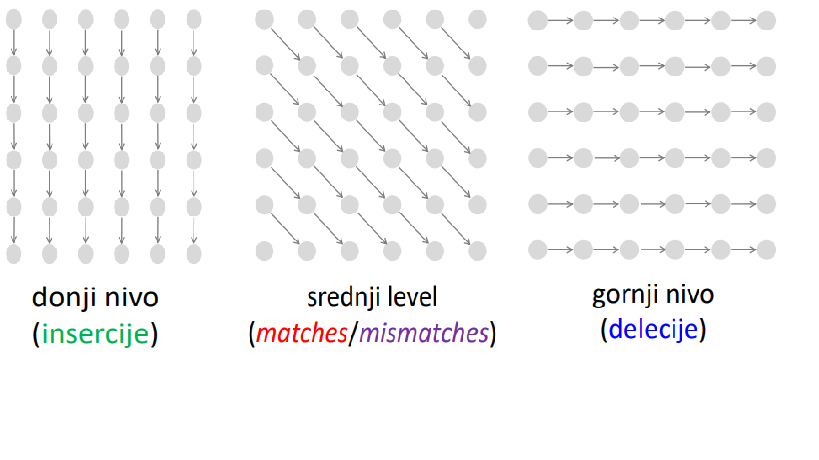
\includegraphics[width=\textwidth]{poglavlja/5/slike/triNivoa.png}
\caption{Podela Menhetna grafa na 3 nivoa}
\label{slika:triNivoa}
\end{figure}
\fi 

Na ovaj način povećali smo broj čvorova, ali smanjen je broj grana, koji je ponovo kvadratan, što nam vraća efikasnost.

\iffalse 
\begin{figure}[h!]
\centering
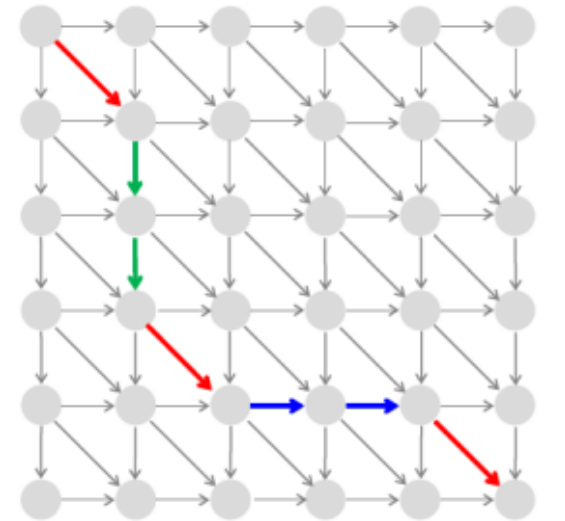
\includegraphics[width=0.5\textwidth]{poglavlja/5/slike/kakoSimulirari.png}
\caption{Kako predstaviti pomoću Menhetn grafa na 3 nivoa?}
\label{slika:kakoSimulirati}
\end{figure}
\fi 

\begin{figure}[h!]
\centering
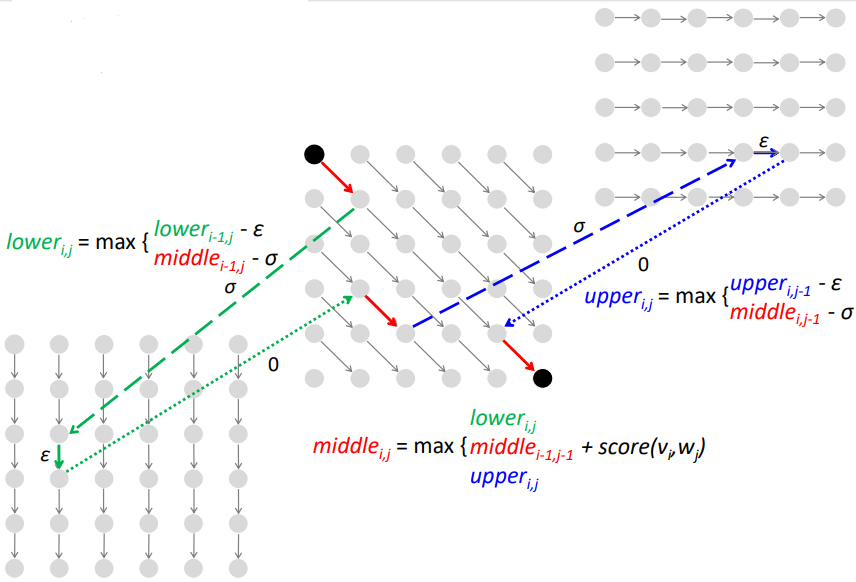
\includegraphics[width=0.7\textwidth]{poglavlja/5/slike/simulacija.png}
\caption{Simulacija Menhetn grafa na 3 nivoa}
\label{slika:simulacija}
\end{figure}

Promenljiva $lower_{i, j}$ računa skor optimalnog poravnanja između $i$-prefiksa niske \texttt{v} i $j$-prefiksa niske \texttt{w} koje se završava delecijom, odnosno, rupom u \texttt{w}. Sa druge strane, promenljiva $upper_{i, j}$ računa skor optimalog poravnanja ovih prefiksa koje se završava insercijom, odnosno, rupom u \texttt{v}. Promenljiva $middle_{i, j}$ računa skor optimalnog poravnanja koje rezultuje pogotkom ili promašajem. U formulama za računanje promeljivih matrica $lower$ i $upper$, prvi red odnosi se na proširenje rupe, dok drugi red predstavlja otvaranje rupe.


\section{Prostorno efikasno poravnanje sekvenci}

Da li možemo poravnati NPR sintetaze iz dve različite bakterije? Uzmimo u obzir sledeće činjenice. NPR sintetaze su obično veoma dugi proteini, približno 20 000 aminokiselina. Vremenska složenost poravnanja je približno jednaka broju ivica (\#edges), odnosno kvadratna. Prostorna složenost poravnanja je približno jednaka broju čvorova (\#nodes), odnosno takođe je kvadratna. Memorija je često usko grlo pri poređenju dugih sekvenci.

Iz prethodnog zaključujemo da nam prostorna složenost pravi problem i da bi za prosečan računar ovo bilo nemoguće da izračuna.  Stoga, potreban nam je drugi pristup koji će nam rešiti problem. Potreban nam je algoritam koji zahteva linearnu prostornu složenost i udvostručenu vremensku složenost. U te svrhe najčešće se koristi algoritam koji radi po principu podeli-pa-vladaj. 


Vraćamo se na graf poravnanja i male nukleotidne sekvence, radi ilustracije. Uvedimo nove pojmove:
\begin{itemize}
    \item Srednja kolona poravnanja (middle) $= \#columns/2$, \ref{slika:srednjaKolona}
    \item Srednji čvor poravnanja - čvor u preseku putanje optimalnog poravnanja i srednje kolone, slika \ref{slika:srednjiCvor}
\end{itemize}

\iffalse 
\begin{figure}[h!]
\centering
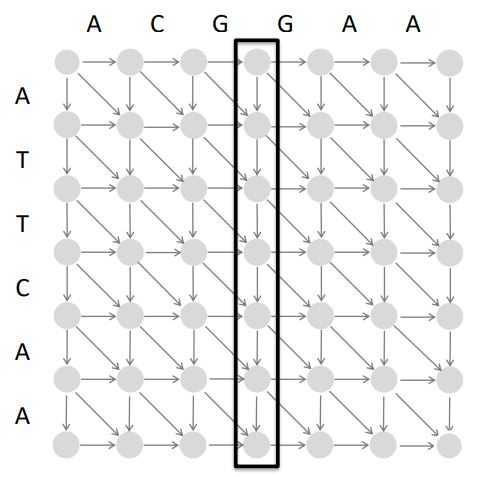
\includegraphics[width=0.5\textwidth]{poglavlja/5/slike/srednjaKolona.JPG}
\caption{Srednja kolona poravnanja}
\label{slika:srednjaKolona}
\end{figure}
\begin{figure}[h!]
\centering
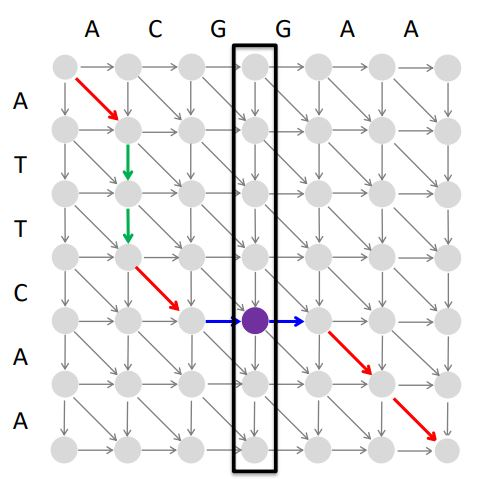
\includegraphics[width=0.5\textwidth]{poglavlja/5/slike/srednjiCvor.JPG}
\caption{Srednji čvor poravnanja}
\label{slika:srednjiCvor}
\end{figure}

\fi 

Koristeći navedene pojmove, demonstrirajmo algoritam \textbf{Podeli-pa-vladaj} za poravnanje sekvenci, slika \ref{slika:podeliPaVladaj}: \\

\begin{lstlisting}
AlignmentPath(source, sink)
    find middleNode
    AlignmentPath(source, middleNode)
    AlignmentPath(middle, sink)
\end{lstlisting}

\begin{figure}[H]
	\begin{minipage}{0.45\textwidth}
		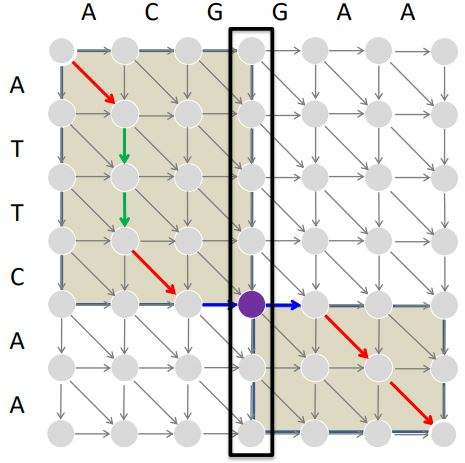
\includegraphics[width=\linewidth]{poglavlja/5/slike/podeliPaVladaj.JPG}
		\caption{Srednja kolona poravnanja}
		\label{slika:podeliPaVladaj}
	\end{minipage}
	\hfill
	\begin{minipage}{0.45\textwidth}
		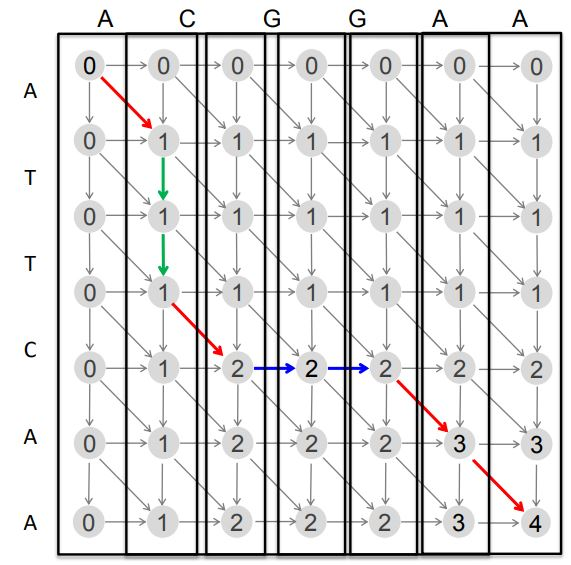
\includegraphics[width=\linewidth]{poglavlja/5/slike/prostornaSlozenost2.JPG}
		\caption{Recikliranje prostora za kolone u grafu poravnanja}
		\label{slika:prostornaSlozenost}
	\end{minipage}
\end{figure}


Za nalaženje najduže putanje u grafu poravnanja traži se čuvanje svih putokaza za - $O(nm)$ prostora. Međutim, za nalaženje dužine najduže putanje u grafu poravnanja ne traži se čuvanje svih putokaza - $O(n)$ prostora, slika \ref{slika:prostornaSlozenost}. Dobijamo da je prostor potreban za algoritam $2*n \sim O(n)$, odnosno, linearan. 

Hoćemo da pokažemo da, da bismo izračunali koliko iznosi dužina najduže putanje, nije potrebno da čuvamo ceo graf, tj. sve njegove čvorove, već je dovoljno da čuvamo samo dve kolone. Prvu kolonu popunimo nulama pa gledamo za drugu kako možemo doći do svakog od čvorova. Kod prvog čvora u toj koloni nema razmišljanja, možemo doći samo horizontalnom granom. Za drugi imamo više izbora, a biramo dijagonalnu granu jer postoji poklapanje. Za sve ostale čvorove ove kolone koristimo vertikalnu granu jer više nema poklapanja koja će uvećati dužinu putanje do nekog od tih čvorova. 

Kao što vidimo, za određivanje težina u drugoj koloni bila nam je potrebna samo jedna prethodna kolona. Kako se krećemo kroz graf, kolonu po kolonu, biće nam potrebna samo prethodna kolona. Pokazali smo da je prostor potreban za podeli-pa-vladaj poravnanje $2*n \sim  O(n)$, odnosno, linearan. Da vidimo kakva će biti vremenska složenost.


Da bismo smanjili prostornu složenost na linearanu, morali smo da se odreknemo kostrukcije najduže putanje. Pitanje je da li, i kako, možemo da nađemo srednji čvor ako ne konstruišemo putanju.

Neka je \textbf{i-putanja} najduža putanja od svih putanja koja posećuje i-ti čvor u srednjoj koloni i neka je \textbf{$length(i)$} dužina i-putanje. Na slici \ref{slika:sourceSink} vidimo da je $length(0)=2$ i $length(4)=4$. Dužinu označavamo sa $length(i)$ i možemo računati po formuli:
\begin{center}
$length(i) = fromSource(i) + toSink(i)$
\end{center}


Na slici \ref{slika:sourceSink} vidimo koliko je potrebno vremena za nalaženje srednjeg čvora - čak $O(nm)$ vremena za nalaženje samo jednog čvora! 



\begin{figure}[H]
	\begin{minipage}{0.55\textwidth}
		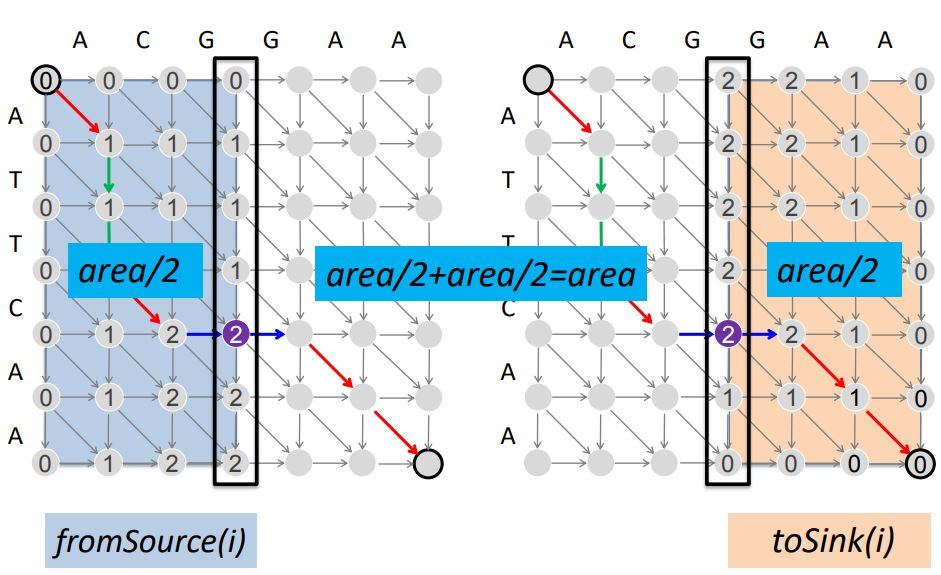
\includegraphics[width=\linewidth]{poglavlja/5/slike/sourceSink.JPG}
		\caption{Računanje vremena za nalaženje srednjeg čvora}
		\label{slika:sourceSink}
	\end{minipage}
	\hfill
	\begin{minipage}{0.35\textwidth}
		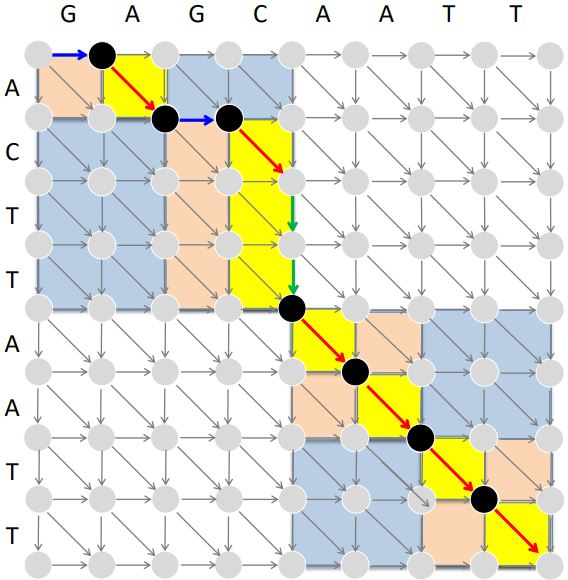
\includegraphics[width=\linewidth]{poglavlja/5/slike/vremenskaSlozenostPPV.JPG}
		\caption{Računanje vremena za nalaženje 7 tačaka}
		\label{slika:vreme}
	\end{minipage}
\end{figure}


Svaki problem se može rešiti u vremenu proporcionalnom broju grana tj. površini koju zauzima. Vreme potrebno za rešavanje naredna dva potproblema: $area/4 + area/4 = area/2$, znači  $O(nm + nm/2)$ vremena za nalaženje 3 čvora. Dakle, vreme potrebno za nalaženje svih čvorova je: $area + area/2 + area/4 + area/8 + \dots < 2 * area$! Slika \ref{slika:vreme} vizuelno prikazuje vreme potrebno za nalaženje 7 tačaka. Pokazali smo da je vremenska složenost $2*n*m \sim O(n*m)$.

\section{Višestruko poravnanje sekvenci}

Do sada su u poravnanju učestvovale samo dve sekvence. Slaba sličnost između dve sekvence postaje značajna ako je prisutna i u drugim sekvencama. Višestruka poravnanja mogu otkriti suptilne sličnosti koje dvostruka poravnanja ignorišu. Na slici \ref{slika:poravnavanjaTriA} je prikazano poravnanje tri A-domena.


\begin{figure}[h!]
\centering
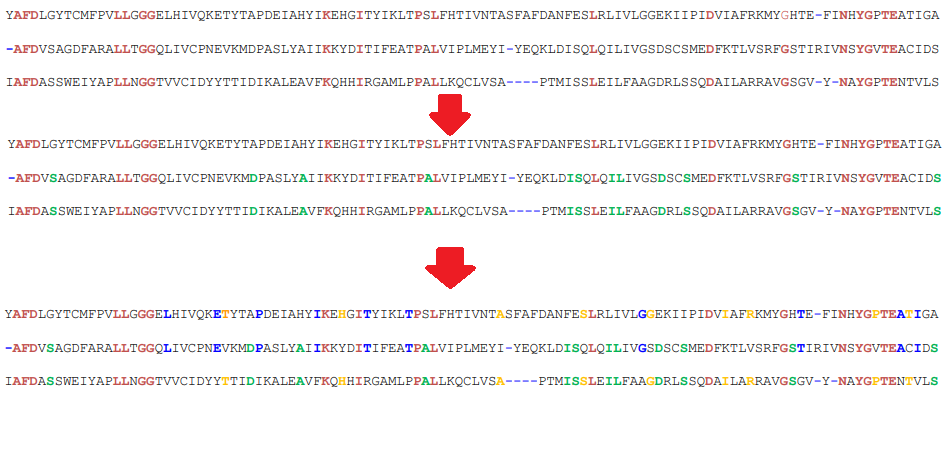
\includegraphics[width=\textwidth]{poglavlja/5/slike/poravnavanjaTriAdomena.png}
\caption{Poravnavanja 3 A-domena}
\label{slika:poravnavanjaTriA}
\end{figure}


Poravnanje 2 sekvence predstavili smo matricom od 2 reda. Tako će poravnanje 3 sekvence biti matrica od 3 reda (slika  \ref{slika:poravnavanjeMatrica}). Na odgovarajuća mesta su ponovo umetnute crtice.

    \begin{figure}[h!]
    \centering
    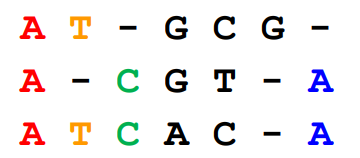
\includegraphics[width=0.3\textwidth]{poglavlja/5/slike/poravnanjeMatrica.png}
    \caption{}
    \label{slika:poravnavanjeMatrica}
    \end{figure}

Funkcija skora treba da dodeljuje visok skor poravnanjima sa konzerviranim kolonama. 




Poravnanje dve niske bilo je predstavljeno mrežom kvadrata. Poravnanje tri sekvence predstavljamo mrežom kockica i govorimo od 3D-putanji. 

Poravnanje sekvenci ATGC, AATC i ATGC predstavljeno je na slici \ref{slika:3d}. Prvo smo napravili matricu od tri reda, a onda posebno obeležili svaki red. Oznake u dodatnim redovima predstavljaju broj simbola do date pozicije u odgovarajućoj niski (crtica se ne računa kao simbol!). Čemu služi to prebrojavanje? 

Ako procitamo sve vrednosti po kolnama, dobićemo 3D putanju, kojom se krećemo od čvora (0, 0, 0) do čvora (4, 4, 4). Kako to izgleda na grafu prikazano je na slici \ref{slika:2d3d}. Ono što je kod dvostrukog poravnanja bilo predstavljeno kvadratom, kod trostrukog poravnanja predstavljeno je kockom. 

\begin{figure}[H]
\centering
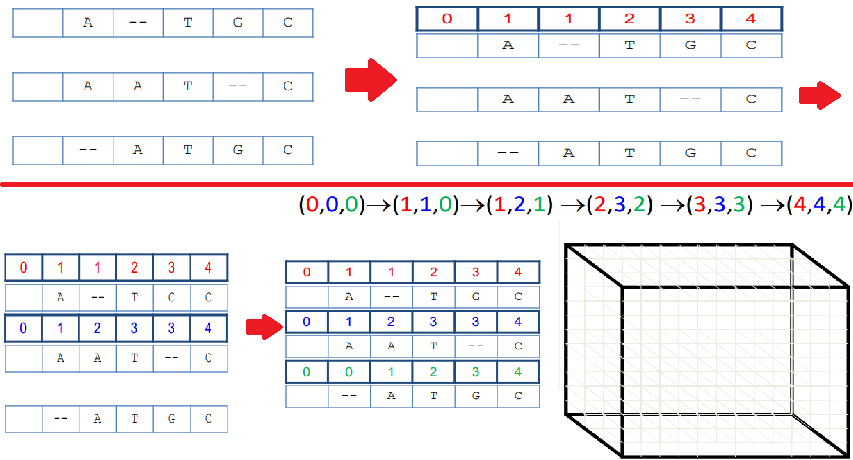
\includegraphics[width=0.8\textwidth]{poglavlja/5/slike/3dPoravnanja.png}
\caption{Poravnanje sekvenci ATGC, AATC i ATGC}
\label{slika:3d}
\end{figure}

\begin{figure}[h]
\centering
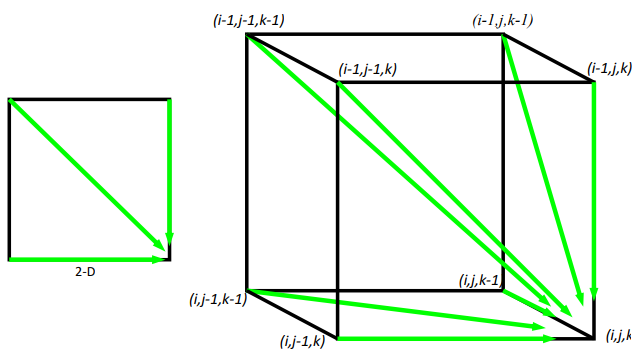
\includegraphics[width=0.5\textwidth]{poglavlja/5/slike/2d3d.png}
\caption{2-D poravnanje u odnosu na 3-D poravnanje}
\label{slika:2d3d}
\end{figure}


Da vidimo kako se rekurentna relacija dinamičkog programiranja za višestruko poravnanje komplikuje sa povećanjem dimenzije:

$s_i,_j,_k$ = $\max$ $\begin{cases}$

$s_{i-1},_{j-1},_{k-1}$+ $\delta(v_i, w_j, u_k)\\$
$s_{i-1},_{j-1},_k$+ $\delta(v_i, w_j, -)\\$
$s_{i-1},_j,_{k-1}$+ $\delta(v_i, -, u_k)\\$
$s_i,_{j-1},_{k-1}$+ $\delta(-, w_j, u_k)\\$
$s_{i-1},_{j},_k$+ $\delta(v_i,-, -)\\$
$s_{i},_{j-1},_k$+ $\delta(-, w_j, -)\\$
$s_{i},_{j},_{k-1}$+ $\delta(-, -, u_k)\\$
$\end{cases}$

gde je $\delta$(x, y, z)  element 3-D matrice skora.

\subsection{Vremenska složenost dinamičkog algoritma za višestruko poravnanje}

Kao kod dvostrukog poravnanja, vremenska složenost je proporcionalna broju grana O(\#edges). Za 3 sekvence n, vremenska složenost je proporcionalna 7$n^3$ (pomoću 7 različitih grana možemo doći do svakog čvora). Za poravnanje $k$ sekvenci, potrebno je izgraditi $k$-dimenzionalni Menhetn graf sa: 
    \begin{itemize}
        \item  $n^k$ čvorova
        \item većina čvorova će imati $2^k - 1$ ulaznih grana
        \item Vremenska složenost: O($2^kn^k$)
    \end{itemize}

Ovo važi ukoliko primenjujemo algoritam globalnog poravnanja na višestruko poravnanje Vidimo da složenost nije najbolja i pitamo se kako to može bolje, efikasnije.
\\
\\
Pogledajmo sledeće. Određujemo trostruko poravnanje. Možemo da primetimo da ono sadrži i neka dvostruka poravnanja. Iz trostrukog poravnanja možemo da izvučemo dvostruka poravanja (\ref{slika:visestrukoDvostruko}). Da li može obrnuto?

\begin{figure}[h!]
\centering
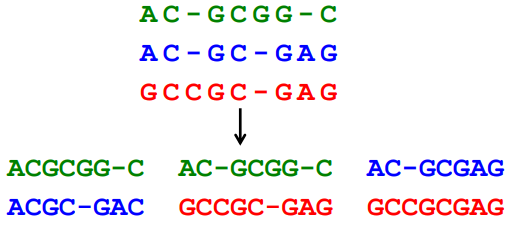
\includegraphics[width=0.5\textwidth]{poglavlja/5/slike/visestrukoDvostruko.png}
\caption{}
\label{slika:visestrukoDvostruko}
\end{figure}

 
Pitamo se, da li za dati skup proizvoljnih dvostrukih poravnanja možemo konstruisati višestruko poravnanje iz kog su izvedeni (slika \ref{slika:dvostruka}).

\begin{figure}[h!]
\centering
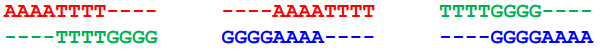
\includegraphics[width=0.7\textwidth]{poglavlja/5/slike/dvostruka.png}
\caption{}
\label{slika:dvostruka}
\end{figure}

Tu će nam pomoći profilna reprezentacija višestrukog poravnanja (slika \ref{slika:profilVisetruko}). Imamo matricu koja ima 5 redova (simboli azbuke i praznina). Broj kolona direktno zavisi od broja kolona u višestrukom poravnanju. Kako popunjvamo matricu? Na isti način kao u poglavlju 2, kada smo pravili profilne matrice motiva. 


\begin{figure}[h!]
\centering
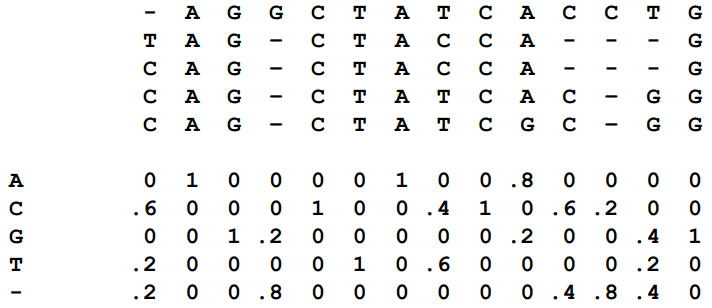
\includegraphics[width=0.6\textwidth]{poglavlja/5/slike/profilVisestruko.png}
\caption{Profilna matrica višestrukog poravnanja}
\label{slika:profilVisetruko}
\end{figure}

Do sada smo poravnavali sekvencu u odnosu na sekvencu. Možemo li poravnati sekvencu u odnosu na profil? Možemo li poravnati profil u odnosu na profil? Predstavićemo jedan od algoritama za višesturko poravnanje koje bi pratilo pohlepni pristup. 

Imamo nekoliko sekvenci. Izabraćemo dve najsličnije sekvence tako što će njihovo dvostruko poravnanje dati najveći skor (poravnaćemo svaku sa svakom). Onda te sekvence kombinjemo u profil i tako smo smanjili broj sekvenci sa $k$ na $k-2$ i jedan profil. Iteriramo postupak dok ne dođemo do zajedničkog profila. 
\\
\\
\noindent\textbf{Primer pohlepnog pristupa:}
\\
\\\noindent Imamo sekvence: GATTCA, GTCTGA, GATATT, GTCAGC koje želimo da poravnamo. Odredićemo 6 dvostrukih poravnanja sa primitivnom šemom skorovanja - poklapanje ima vrednost 1, dok promašaj i indel-i imaju vrednost -1 (slika \ref{slika:sestDvostrukih}).

\begin{figure}[h]
	\begin{minipage}{0.55\textwidth}
		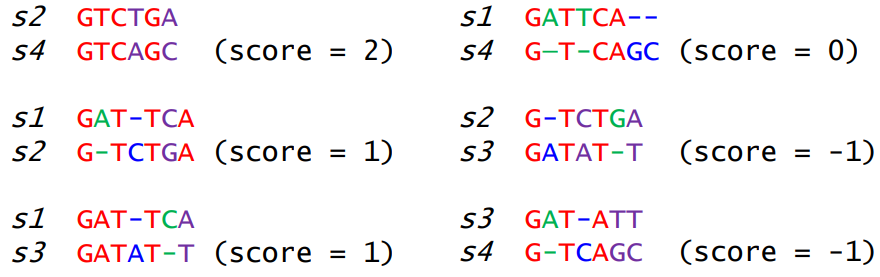
\includegraphics[width=\linewidth]{poglavlja/5/slike/sestDvostrukih.png}
		\caption{}
		\label{slika:sestDvostrukih}
	\end{minipage}
	\hfill
	\begin{minipage}{0.35\textwidth}
		\includegraphics[width=\linewidth]{poglavlja/5/slike/profil.png}
		\caption{}
		\label{slika:profil}
	\end{minipage}
\end{figure}

Pošto su $s_2$ i $s_4$ najbliže, od njih pravimo profil. Kako pravimo profil? Tamo gde smo imali poklapanja, ti karakteri ostaju nepromenjeni. Gde ima nepoklapanja, oba uvrstimo na to mesto (prikaz na slici \ref{slika:profil}). Time smo dobili novi skup od 3 sekvence za poravnanje: $s_1$ = GATTCA, $s_3$ = GATATT i $s_2,_4$ = \textcolor{black}{GTC}\textcolor{black}{t/a}\textcolor{black}{G}\textcolor{black}{a/c}

\iffalse

\newpage
\section{Zadaci sa vežbi}
\setexamplecodestyle

U nastavku će biti predstavljeni zadaci sa vežbi na kursu rađeni u programskom jeziku Python.

\subsection{Manhattan Tourist}

\lstinputlisting[language=Python]{poglavlja/5/kodovi/ManhattanTourist.py}

\subsection{LCS Backtrack}

\lstinputlisting[language=Python]{poglavlja/5/kodovi/LCSBacktrack.py}

\subsection{Global Alignment}

\lstinputlisting[language=Python]{poglavlja/5/kodovi/GlobalAlignment.py}

\subsection{Local Alignment}

\lstinputlisting[language=Python]{poglavlja/5/kodovi/LocalAlignment.py}

\subsection{Edit Distance}

\lstinputlisting[language=Python]{poglavlja/5/kodovi/EditDistance.py}
\fi 
